\chapter{}\label{ch:aufg6}

Es soll eine Schrittmotorsteuerung implementiert werden im entsprechenden Statechart des Simulink-Modells. \\
Um die Ansteuerung variabel zu halten, wurde das entsprechende Statechart im Simulink-Modell am Laborrechner angepasst, dies ist in Abbildung \ref{fig:6:simulink} zu sehen. Der zeitliche Verlauf der internen Ansteuerung wird in Abbildung \ref{fig:6:messung} dargelegt.

\begin{figure}[h]
	\centering
	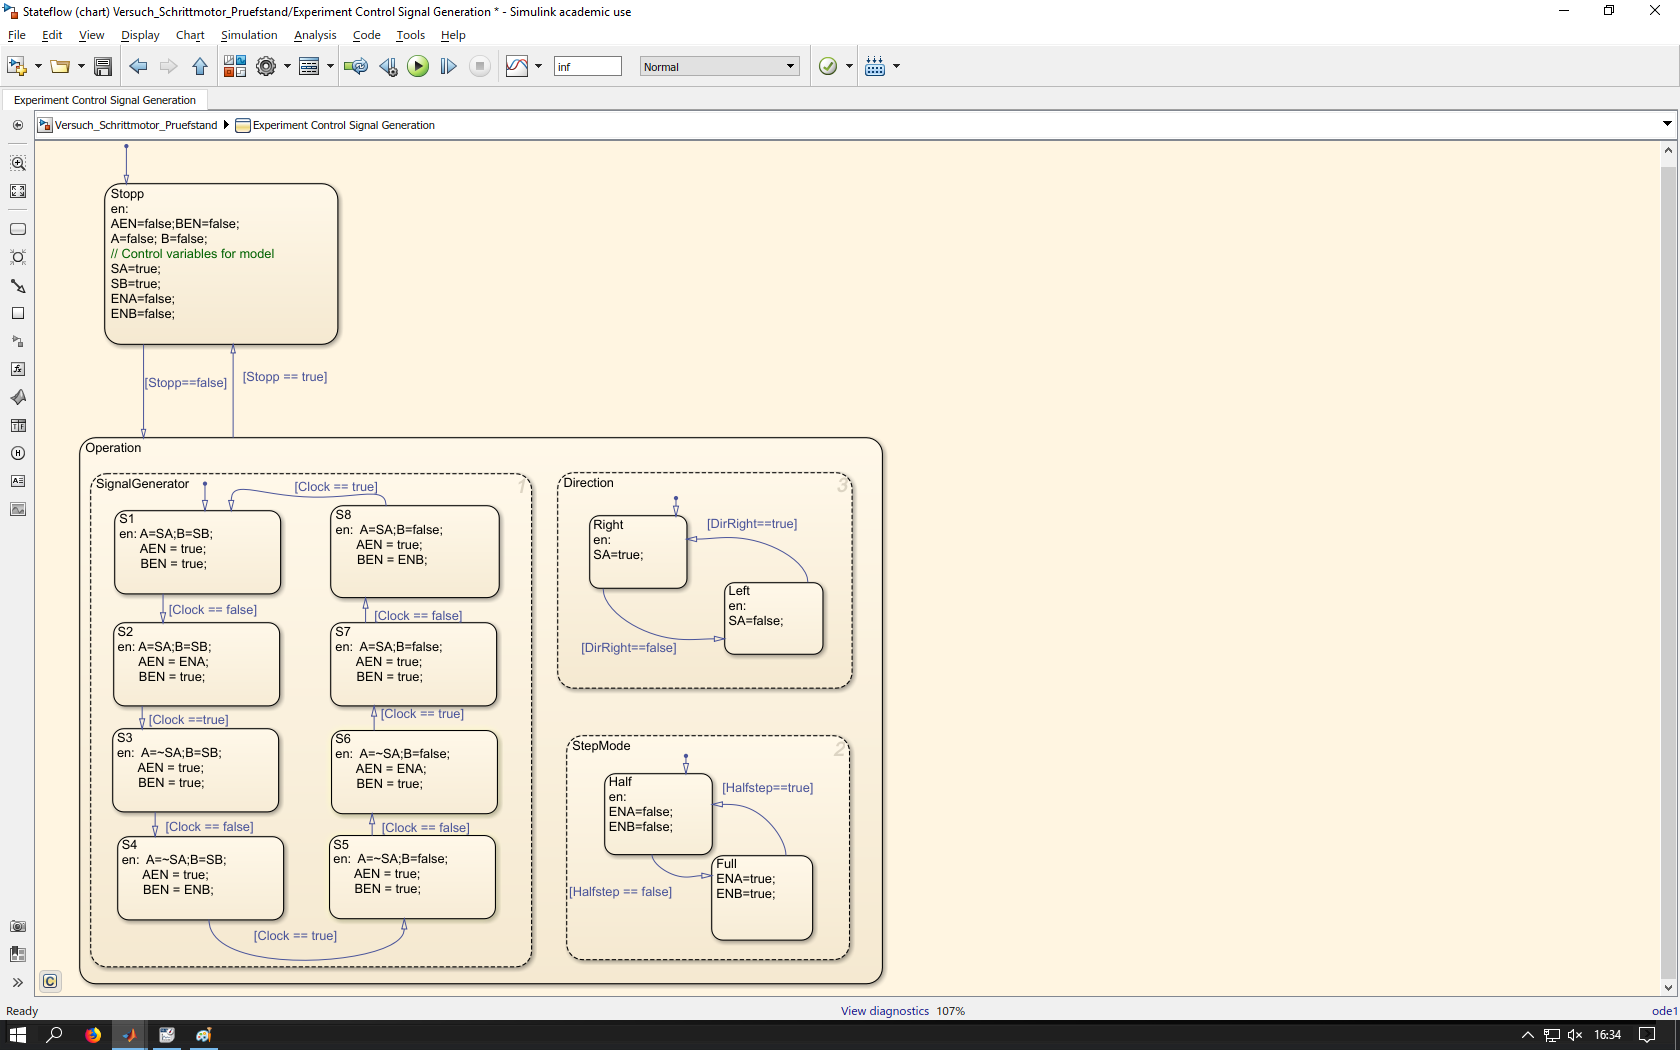
\includegraphics[width=0.6\textwidth]{./Bilder/2.png}
	\caption{Matlab-Simulink Modell der Ansteuerung des Schrittmotors}
	\label{fig:6:simulink}
\end{figure}


\begin{figure}[h]
	\centering
	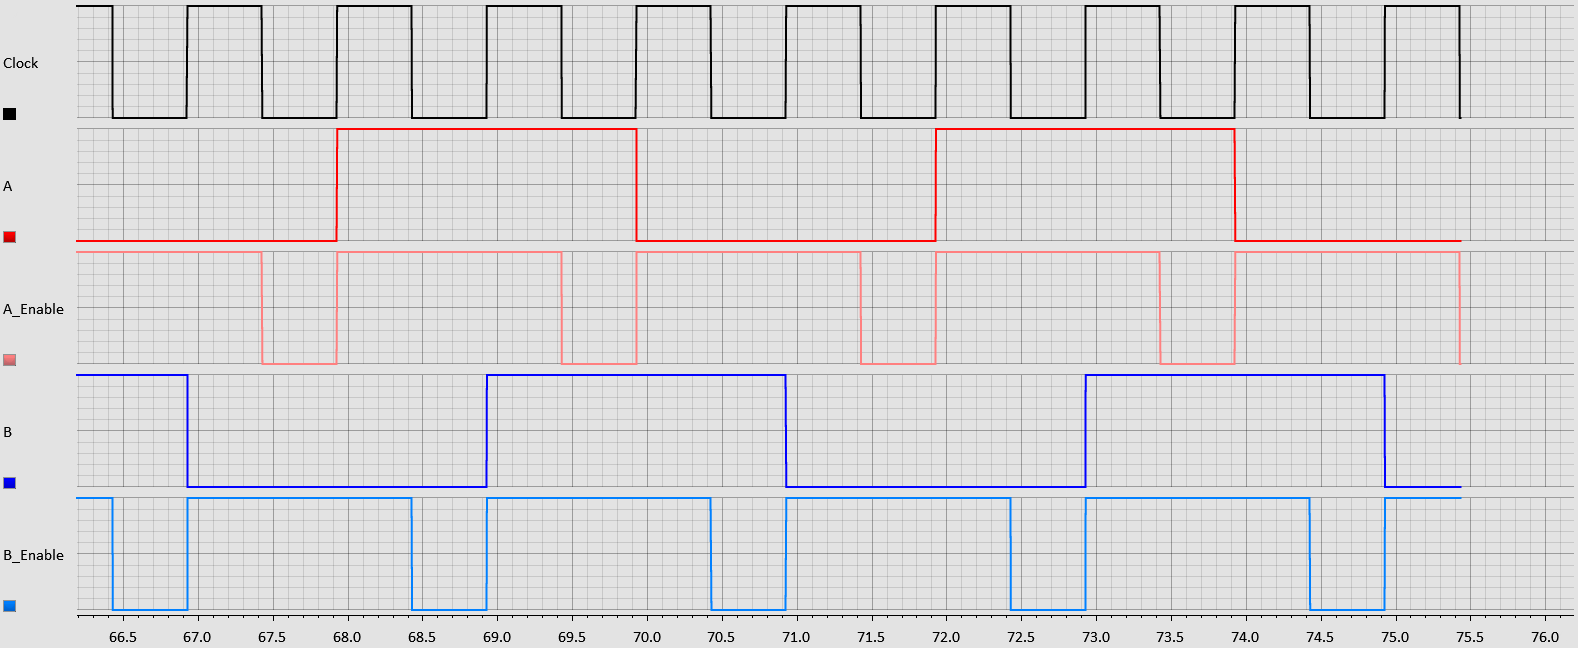
\includegraphics[width=0.6\textwidth]{./Bilder/1.png}
	\caption{Verläufe der Ansteuerungssignale}
	\label{fig:6:messung}
\end{figure}